
\documentclass[11pt]{article}
\usepackage[paper=letterpaper, margin=.5in]{geometry}
\pdfpagewidth 8.5in
\pdfpageheight 11in
\setlength\parindent{0in}

%% AMS PACKAGES - Chances are you will want some or all of these if writing a math dissertation.
\usepackage{amsmath, amscd, amssymb, amsthm, multirow, enumerate, multicol, graphicx, listings}
\newcommand{\Z}{\mathbb{Z}}
\newcommand{\R}{\mathbb{R}}
\newcommand{\Q}{\mathbb{Q}}
\newcommand{\C}{\mathbb{C}}
\newcommand{\N}{\mathbb{N}}
\newcommand{\V}{\mathbb{V}}
\newcommand{\U}{\mathcal{U}}
\newcommand{\del}{\partial}
\newcommand{\real}{\textrm{Re }}
\newcommand{\imag}{\textrm{Im }}
\newcommand{\pd}[2]{\frac{\partial #1}{\partial #2}}
\newcommand{\deriv}[2]{\frac{d #1}{d #2}}
\newcommand{\sumk}{\sum_{k=1}^\infty}
\newcommand{\sumj}{\sum_{j=1}^\infty}
\newcommand{\sumn}{\sum_{n=0}^\infty}
\newcommand{\summ}[2]{\sum_{k=#1}^{#2}}
\newcommand{\sig}[1]{\sum_{#1 =1}^\infty}
\newcommand{\un}[1]{\bigcup_{#1 =1}^\infty}
\newcommand{\inter}[1]{\bigcap_{#1 =1}^\infty}
\newcommand{\ip}[2]{\langle #1, #2 \rangle}
\newcommand{\ipxu}{\langle x,u_j \rangle}
\newcommand{\uj}{\{u_j\}_{j=1}^\infty}
\newcommand{\B}{\mathcal{B}}

\newcommand{\E}{\mathrm{E}}
\newcommand{\var}{\mathrm{Var}}
\newcommand{\cov}{\mathrm{Cov}}
\newcommand{\ST}{mbox{ s.t. }}

\newcommand{\Example}{\noindent {\bf Example. \quad} }
\newcommand{\Proof}{\noindent {\bf Proof: \quad} }
\newcommand{\Remark}{\noindent {\bf Remark. \quad} }
\newcommand{\Remarks}{\noindent {\bf Remarks. \quad} }
\newcommand{\Case}{\noindent {\underline{Case} \quad} }

\newcommand{\st}{ \; \big | \:}

\newcommand{\deuc}{d_{\mathrm euc}}
\newcommand{\dtaxi}{d_{\mathrm taxi}}
\newcommand{\ddisc}{d_{\mathrm disc}}
\newtheorem{theorem}{Theorem}[section]
\newtheorem{lemma}[theorem]{Lemma}
\newtheorem{proposition}[theorem]{Proposition}
\newtheorem{corollary}[theorem]{Corollary}
\theoremstyle{definition}
\newtheorem{definition}[theorem]{Definition}
\newtheorem{example}[theorem]{Example}

\begin{document}
%%%%%%%%%%%%%%%%%%%%%%%%%%%%%%%%%%%%%%%%%%%%%%%%%%%%%%%%%%%%%%%%%%%%%%%%%%%%%%%%%%%%%%%%%%%%%%%%%%%%%%%%%%%%%%%%%%%%%%%%%%%%%%%%%%%%%

Homework 2 \hfill Aaron Maurer
\vspace{2mm}
\hrule
\vspace{2mm}
\begin{itemize}
    \item[1.]
        \begin{itemize}
            \item[a)]
                \begin{align*}
                    \E[\hat{\beta} \vert X] &= \E[(X'X)^{-1}X'Y \vert X] \\
                                            &= \E[(X'X)^{-1}X'(X\beta+e) \vert X] \\
                                            &= \E[(X'X)^{-1}X'X\beta+(X'X)^{-1}X'e \vert X] \\
                                            &= \E[\beta \vert X] + (X'X)^{-1}X' \E[e \vert X] \\
                                            &= \beta + (X'X)^{-1}X' b(X)
                \end{align*}
                Thus, $\hat{\beta}$ is only unbiased when \((X'X)^{-1}X' b(X) = 0\).
                In other words, $\hat{\beta}$ is biased if  $b(X)$ is in the span of \((X'X)^{-1}X'\).
            \item[b)]
                \begin{align*}
                    \var[\hat{\beta} \vert X ] &= \var[(X'X)^{-1}X'Y \vert X ] \\
                                               &= \var[(X'X)^{-1}X'(X\beta+e) \vert X ] \\
                                               &= \var[(X'X)^{-1}X'X\beta+(X'X)^{-1}X'e \vert X] \\
                                               &= \var[\beta+(X'X)^{-1}X'e \vert X] \\
                                               &= \var[(X'X)^{-1}X'e \vert X] \\
                                               &= (X'X)^{-1}X'\var[e \vert X]((X'X)^{-1}X')' \\
                                               &= (X'X)^{-1}X'\sigma^2I X (X'X)^{-1} \\
                                               &= (X'X)^{-1}X'X(X'X)^{-1} \sigma^2 \\
                                               &= (X'X)^{-1}\sigma^2 \\
                \end{align*}
                Thus, though $\hat{\beta}$ may be biased, it has no higher variance with assumption A2$'$ than with the usual assumption A2.
        \end{itemize}
    \item[2.]
        \begin{itemize}
            \item[i.]
                Given that the variable \(wt_i = \beta_0 + e_i\), where each $e_i$ is normally distributed around $0$ and independent of all other $e_j$ such that $j\neq i$, and independent of the variable height, the probability that a model that included height would reduce the residual sum of squares as much as it has or more is $17.31\%$.
            \item[ii.]
                Given that the variable \(wt_i = \beta_0 + \beta_1 ht_i + e_i\), where each $e_i$ is normally distributed around $0$ and independent of all other $e_j$ such that $j\neq i$, the probability that \(\vert \hat\beta_0 \vert \geq 36.8759 \) given a null hypothesis that \(\beta_0=0\) is $58.3\%$.
           \item[iii.]
               Given that the variable \(wt_i = \beta_0 + \beta_1 ht_i + e_i\), where each $e_i$ is normally distributed around $0$ and independent of all other $e_j$ such that $j\neq i$, the probability that \(\vert \hat\beta_1 \vert \geq .5821  \) given a null hypothesis that \(\beta_1=0\) is $17.3\%$.
            \item[iv.]
                You can not compute the probability of the fitted model being the right one, only the probability of seeing the given data and estimates on it for various assumptions of the underlying process that generated it.
        \end{itemize}
    \item[3.]
        All the individuals formulas for the desired quantities are: \\
        \[SSreg = \frac{R^2 RSS}{1 - R^2}= \frac{.2084 \times 351191.4}{1-.2084}=92456.14\]
        \[RSS=(RSE \times df)^2=(2.993 \times 198)^2=351191.4\]
        \[MSreg = \frac{SSreg}{regDF} = \frac{92456.14}{1}= 92456.14\]
        \[\hat\sigma^2 = \frac{RSS}{resDF} = \frac{351191.41}{198} = 1773.694\]
        \[F = \frac{MSreg}{\hat\sigma^2} = \frac{92456.14}{1773.694} = 1773.694 \]
        Which fit in the table as such: \\
        \begin{tabular}{l | l l l l l}
            Regression & df      & ss               & ms       & F     \\
            \hline
            Regression & regDF = 1       & SSreg = 92456.14 & MSreg = 92456.14          & F = 52.126 \\
            Residual   & resDf = 198     & RSS = 351191.4   & $\hat\sigma^2$ = 1773.694 &  
        \end{tabular}
    \item[4.]
        \begin{itemize}
            \item[a)] These are the resulting confidence intervals: \\
                \begin{tabular}{l | r l r l}
                    Confidence Level & $\beta_0$ LB & $\beta_0$ UB & $\beta_1$ LB & $\beta_1$ UP \\
                    \hline
                    66\%             &       (3.802,& 3.828)       &       (-.062,& -.059)     \\
                    90\%             &       (3.792,& 3.837)       &       (-.063,& -.058)     \\
                    95\%             &       (3.788,& 3.841)       &       (-.064,& -.057)
                \end{tabular}
            \item[b)] We get the variance estimate:
            \[1.538\times10^{-5} = \sigma^2 \left[ \begin{array}{c c} 1 & 10 \end{array} \right] \left(X'X\right)^{-1} \left[ \begin{array}{c} 1 \\  10 \end{array} \right] \]
            \item[c)] This is what we end up with, for a 95\% CI: \\
                \begin{tabular}{l | r c l}
                    Type       & LB    & Fit   & UB    \\
                    \hline
                    Mean       & 3.005 & 3.022 & 3.038 \\
                    Prediction & 2.800 & 3.022 & 3.245 
                \end{tabular}
            \item[d)]
                The confidence interval is smallest near the mean of fixed acidity ($8.31$ in the data set). This stands to reason, since the confidence intervals are based on conditioned slices of a multivariate normal distribution; these slices will be steepest towards the center of the distribution (around the means of all variables), and flattest in the tails. In other words, its harder to screw up a prediction where you have a lot of data than where you don't have much data. \\
                \begin{center}
                    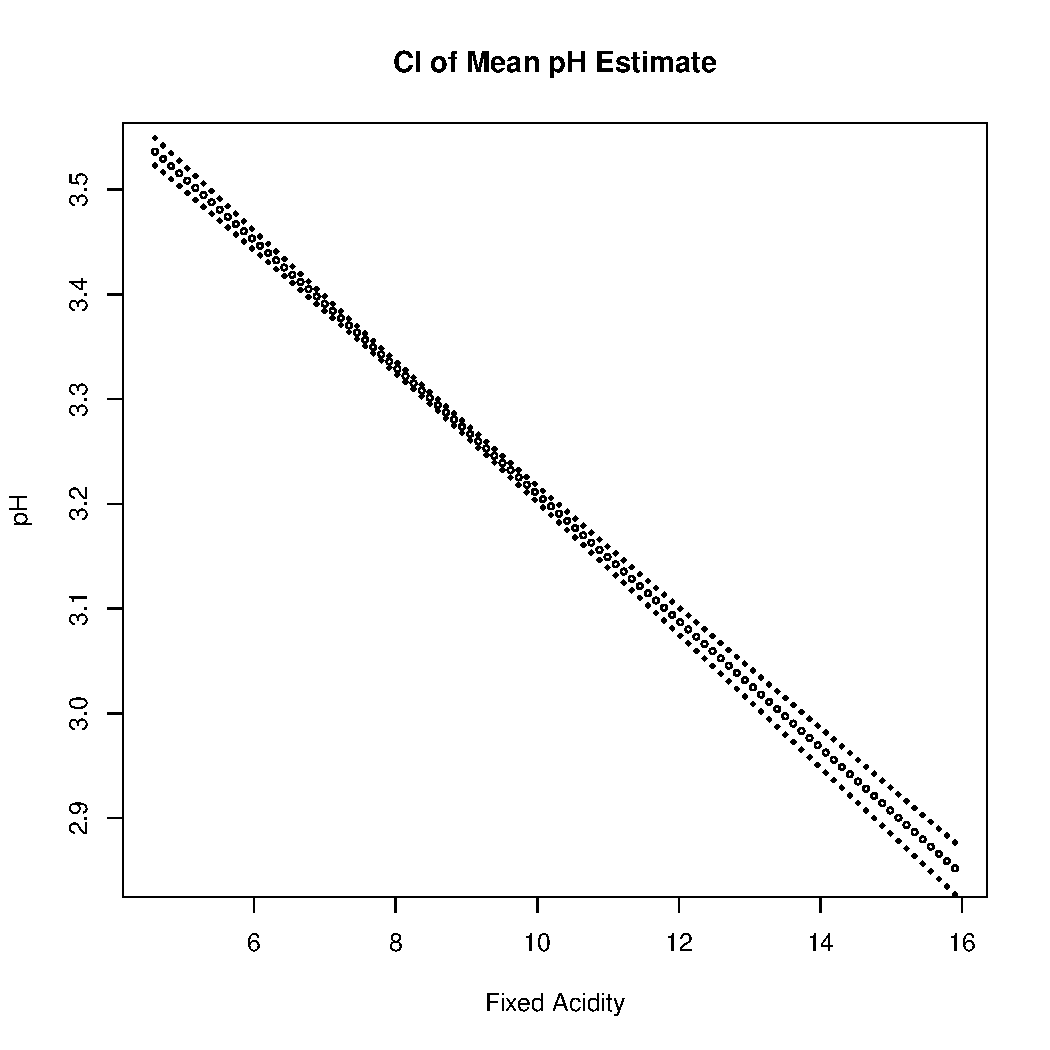
\includegraphics[width=12cm]{hw2_plot} 
                \end{center}
        \end{itemize}
        Here is my R code: \\
        \lstinputlisting{hw2.R}
\end{itemize}
\end{document}
